\section{Messwerte}

\begin{table}
  \centering
  \caption{gemessene Maßen der Kugeln}
  \label{tab:Kugeldaten}
  \begin{tabular}{c c c c c c}
    \toprule $m_{gr} \,\, in \,\, \symup{g}$  & $m_{kl} \,\, in \,\, \symup{g}$ &
             $d_{gr} \,\, in \,\, \symup{cm}$ & $ \increment d_{gr} \,\, in \,\, \symup{cm}$ &
             $d_{kl} \,\, in \,\, \symup{cm}$ & $ \increment d_{kl} \,\, in \,\, \symup{cm}$ \\
    \midrule 4.96 & 4.46 & 1.56 & 0.00 & 1.54 & 0.00
  \end{tabular}
\end{table}

\begin{table}
  \centering
  \caption{gemessene Werte für die Fallzeit der kleinen und großen Kugel}
  \label{tab:Messdaten}
  \begin{tabular}{c c}
    \toprule $Fallzeit \,\, Kugel \, 2 \,\, in \,\, \symup{s}$ &
             $Fallzeit \,\, Kugel \, 1 \,\, in \,\, \symup{s}$ \\
    \midrule
    11.80 & 68.47  \\
    11.80 & 68.95  \\
    12.15 & 68.69  \\
    11.73 & 68.53  \\
    12.21 & 68.50  \\
    11.47 & 67.69  \\
    12.10 & 68.83  \\
    11.96 & 68.41  \\
    11.86 & 68.38  \\
    11.87 & 68.60  \\
    \bottomrule
  \end{tabular}
\end{table}

\begin{table}
  \centering
  \caption{gemessene Werte für die große Kugel}
  \label{tab:Messdaten2}
  \begin{tabular}{c c c }
    \toprule  $Temperatur \,\, in \,\, \symup{°C}$ & $Messung \, 1 \,\, in \,\, \symup{s}$ &
              $Messung \, 2 \,\, in \,\, \symup{s}$ \\
    \midrule
    31.0 & 68.86 & 68.86 \\
    36.0 & 68.33 & 68.21 \\
    39.0 & 65.75 & 65.76 \\
    45.0 & 60.32 & 60.52 \\
    49.5 & 59.27 & 59.27 \\
    51.5 & 58.52 & 58.66 \\
    56.0 & 58.30 & 58.29 \\
    60.0 & 56.60 & 56.72 \\
    64.0 & 55.10 & 55.15 \\
    68.0 & 54.35 & 54.40 \\
    \bottomrule
  \end{tabular}
\end{table}

\begin{table}
  \centering
  \caption{Mittelwerte der Fallzeiten für Teil 1 des Versuches}
  \begin{tabular}{c c c c}
    \toprule $Fallzeit \,\, Kugel \,\, 1 \,\, in \,\, \symup{s}$ & $\increment t \,\, in \,\, \symup{s}$ &
             $Fallzeit \,\, Kugel \,\, 2 \,\, in \,\, \symup{s}$ & $\increment t \,\, in \,\, \symup{s}$ \\
    \midrule
    68.51 & 0.11 & 11.90 & 0.07 \\
    \bottomrule
  \end{tabular}
  \label{tab:FallzeitenGemittelt}
\end{table}

\begin{table}
  \centering
  \caption{Mittelwerte der Messung bei verschiedenen Temperaturen für die große Kugel}
  \label{tab:TemperaturGemittelt}
  \begin{tabular}{c | c c c c c c c c c c }
    \toprule
    $Temperatur \,\, in \,\,\symup{K}$          & 304.15 & 309.15 & 312.15 & 318.15 & 322.65 \\
    $Fallzeit \,\, in \,\,\symup{s}$            & 68.86 & 68.27 & 65.76 & 60.42 & 59.27 \\
    $\increment t_1 \,\, in \,\,\symup{s}$     & 0.00 & 0.06 & 0.01 & 0.10 & 0.00 \\
    \midrule
    $Temperatur \,\, in \,\, \symup{K}$          & 324.65 & 329.15 & 333.15 & 337.15 & 341.15 \\
    $Fallzeit \,\, in \,\, \symup{s}$           & 58.59 & 58.30 & 56.66 & 55.13 & 54.38 \\
    $\increment t_2 \,\, in \,\, \symup{s}$     & 0.07 & 0.01 & 0.06 & 0.03 & 0.03 \\
    \bottomrule
  \end{tabular}
\end{table}

\newpage

\section{Auswertung}

\subsection{Bestimmung der Apparatekonstante für die große Kugel}

In dem ersten Teil des Versuches soll die Apparatekonstante für die große Kugel
(Kugel 1) bestimmt werden. Dafür wird mithilfe der bekannten Apparatekonstante
für die kleine Kugel (Kugel 2) die Viskosität des Wassers bei Raumtemperatur
bestimmt und in folgende Formel eingesetzt:

\begin{align}
  \label{eqn:KappaGroß}
  \Kappa_{kl} &= 0.07640 \, \symup{mPa\, cm^3 / g} \\
  \eta        &= \Kappa_{gr} \cdot \left( \rho_K - \rho_{Fl} \right) \cdot t
\end{align}

Bei $\rho_K$ und $\rho_{Fl}$ handelt es sich um die Dichten der Kugel und der betrachteten
Flüssigkeit. Mithilfe der gemessenen Durchmesser und Gewichte der Kugeln kann die Dichte
mit folgenden Formeln bestimmt werden:

\begin{align}
  r               &= \frac{d}{2} \\
  \rho            &= \frac{m}{\frac{4}{3} \cdot \pi \cdot r^2} \\
  \increment \rho &= \sqrt{ \left(\partial_m \rho \cdot \increment m \right) ^2 +
                    \left( \partial_r \rho \cdot \increment r \right) ^2}
\end{align}

\begin{align}
  r_{gr}    &= (0.78017 \pm 0.00017) \, \symup{cm}     & r_{kl}    &= (0.77167 \pm 0.00017) \, \symup{cm} \\
  \rho_{gr} &= (2.4936 \pm 0.0016) \, \symup{g/cm^3} & \rho_{kl} &= (2.3120 \pm 0.0015) \, \symup{g/cm^3} \\
  \rho_{W}  &= 0.998 \, \symup{g/cm^3}
  \label{eqn:Daten}
\end{align}

Die Dichte für das Waser wurde dabei \cite{Kohlrausch} entnommen. In Tabelle
\ref{tab:FallzeitenGemittelt} sind die Mittelwerte und Fehler der gemessenen
Fallzeiten für die kleine und Große Kugel bei Raumtemperatur eingetragen.
Somit ergibt sich für $K_{gr}$ folgender Wert:

\begin{align}
  \Kappa_{gr} &= \frac{K_{kl} \cdot \left( \rho_{kl} - \rho_{w} \right) \cdot t_{kl}}{\left( \rho_{gr} - \rho_{w} \right) \cdot t_{gr}} \\
              &= (0.01165 \pm, 0.00007) \, \symup{mPa\, cm^3 / g}
\end{align}

Der Fehler für $\Kappa_{gr}$ ergeben sich mit der Gaußschen Fehlerfortpflanzung:

\begin{align}
\increment K_{gr} &= \sqrt{ \left( \partial_{t_{kl}} K_{gr} \cdot \increment t_{kl} \right)^2 +
                            \left( \partial_{t_{gr}} K_{gr} \cdot \increment t_{gr} \right)^2 +
                            \left( \partial_{\rho_{kl}} K_{gr} \cdot \increment \rho_{kl} \right)^2 +
                            \left( \partial_{\rho_{gr}} K_{gr} \cdot \increment \rho_{gr} \right)^2 }
\end{align}

\begin{table}
  \centering
  \caption{Werte der Viskositäten für experimentell bestimmte Werte}
  \label{tab:nuExp}
  \begin{tabular}{c c c}
    \toprule $Temperatur \,\, in \,\, \symup{K}$ & $\eta_{ex} \,\, in \,\, \symup{ mPa s}$ &
            $\increment \eta_{ex} \,\, in \,\, \symup{mPa} \, \symup{s}$   \\
    \midrule
    304.15 & 1.202 & 0.007 \\
    309.15 & 1.193 & 0.007 \\
    312.15 & 1.151 & 0.007 \\
    318.15 & 1.059 & 0.007 \\
    322.65 & 1.040 & 0.006 \\
    324.65 & 1.021 & 0.006 \\
    329.15 & 1.024 & 0.006 \\
    333.15 & 0.997 & 0.006 \\
    337.15 & 0.972 & 0.006 \\
    341.15 & 0.961 & 0.006 \\
    \bottomrule
  \end{tabular}
\end{table}

\begin{table}
  \centering
  \caption{Werte der Viskositäten für Literaturwerte}
  \label{tab:nuLit}
  \begin{tabular}{c c c c c c}
    \toprule
    $Temperatur \,\, in \,\, \symup{K}$       & 303.15 & 313.15 & 323.15 & 333.15 & 143.15 \\
    $\eta_{lit} \,\, in \,\, \symup{ mPa s}$  & 0.7977 & 0.6531 & 0.5471 & 0.4668 & 0.4045 \\
    \bottomrule
  \end{tabular}
\end{table}

\begin{figure}
  \centering
  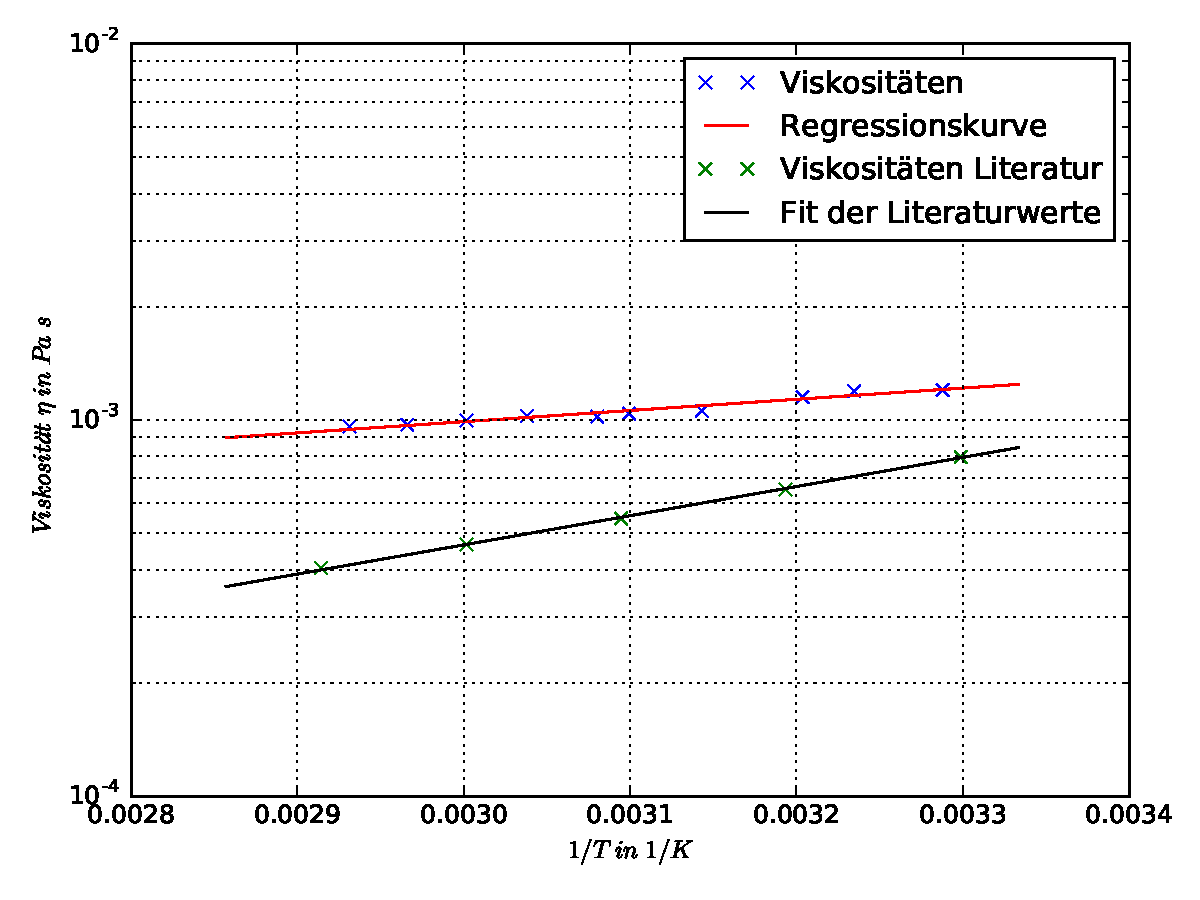
\includegraphics[height = 9.5 cm]{Plot_T_1.pdf}
  \caption{ln(\texorpdfstring{$\eta$}{i}) gegen 1/T, Daten aus Tabellen \ref{tab:nuExp} und \ref{tab:nuLit}}
  \label{plt:Viskos_T}
\end{figure}

\subsection{Bestimmung der Konstanten A/B für die zeitabhängige Viskosität \texorpdfstring{$\eta(T)$}{z}}

In der Abbildung \ref{plt:Viskos_T} sieht man den Logarythmus von $\eta$ aufgetragen
gegen T. Mithilfe einer linearen Regression mit der folgenden Formel können nun
die Parameter der Andradeschen Gleichung bestimmt werden:

\begin{align}
  \eta(T)   &= A \cdot \exp(\frac{B}{T})\\
  ln (\eta) &= ln (A) + B \cdot \frac{1}{T}
\end{align}

Damit ergeben sich für die Parameter A und B folgende Werte

\begin{align}
  \symup{A} &= (0.131 \pm 0.022) \symup{mPa s}\\
  \symup{B} &= (673 \pm 30) \, \symup{K}
\end{align}

\subsection{Bestimmung der Reynoldszahl}

Mithilfe der Formel für die Reynoldszahl \eqref{eqn:Reynolds Zahl} kann bei dem
vorliegenden Versuch beurteilt werden, ob es sich um eine laminare Strömung handelt.
Als kritische Zahl für Rohrströmungen gilt normalerweise ein Faktor von ca. 2300.
Da für das $d$ in diesem Fall jedoch nicht der Querschnitt der Strömung, sondern
der Durchmesser der umströmten Kugel verwendet wird, halbiert sich dieser Wert zu
$Re_{krit} = 1150$. \cite{Reynold}

Mit dem in \eqref{eqn:Daten} berechneten Radien der Kugeln und der Dichte von Wasser
für die jeweiligen Temperaturen ergeben sich für die Reynoldzahlen nun folgende
Werte:

\begin{table}
  \caption{Reynoldszahlen der großen Kugel für die verschiedenen Temperaturen}
  \label{tab:Reynolds}
  \begin{tabular}{c | c c c c c c c c c c }
    \toprule
    $Temperatur \,\, in \,\, \symup{°C}$ & 31 & 36 & 9 & 45 & 49.5 & 51.5 & 56 & 60 & 64 & 68 \\
    \midrule
    $Re$                            & 18.8 & 19.0 & 20.5 & 24.2 & 25.0 & 26.0 & 25.8 & 27.1 & 28.6 & 29.2 \\
    $\increment Re $                & 0.2 & 0.2 & 0.2 & 0.3 & 0.3 & 0.3 & 0.3 & 0.3 & 0.3 & 0.3 \\
    \bottomrule
  \end{tabular}
\end{table}

Und mit der gleichen Berechnung ergibt sich für die kleine Kugel ein Wert von:

\begin{equation}
  Re_{kl} = (12.90 \pm 0.08)
\end{equation}

\section{Diskussion}

Wie man in den Abbildungen \ref{plt:ViskosT} und \ref{plt:Viskos_T} erkennen kann,
weichen die ermittelten Viskositäten für destilliertes Wasser deutlich von den
Literaturwerten ab. Durch einen Fit der Literaturwerte an die Andradesche Gleichung
ergeben sich die Parameter $ A = 2.19 \cdot 10^{-6} $ und $ B = 1.79 \cdot 10^{3} $.
Im Durchschnitt weichen die Funktionen um ca. $ 0.000495 \, \symup{Pa \, s}$ ab.
Jedoch ist auch erkennbar, dass das Verhalten beider Funktionen sich ähnelt, somit
kann ein systematischer Fehler als ziemlich wahrscheinlich angenommen werden.

Die ermittelten Reynoldszahlen lassen sich schlecht mit Literaturwerten vergleichen,
da sie für jedes Experiment aufgrund der Abhängigkeiten von Apparaturwerten
unterschiedlich sind. Allerdings sind die ermittelten Reynoldszahlen deutlich
kleiner als der in Abschnit 4.2 angegebene kritische Wert $R_{krit} = 1150$.
Somit handelt es sich mit einer ziemlich großen Sicherheit bei dem beobachteten
Experiment um laminare Strömungen.

Die entstandenen Abweichungen für die Viskositäten sind vermutlich auf statistischen
Fehler zurückzuführen. Ein großer Faktor war vermutlich die Zeitmessung bei dem
Experiment. Hier ist einerseits die menschliche Reaktionszeit mit einzubeziehen
und andererseist ist die gemessenen Zeiten auch davon abhängen, ob man beim Start
und Ende jeder Messungjeweils den selben Referenzpunkt der Kugel beobachtet, was
in der Praxis schwer exakt zu realisieren ist.
